\section{Calibration of a Cosmic Ray Tagger module}
While time resolution of the \gls{crt} can be calibrated without directly knowing the gain, calibrating the latter is critical for position resolution and efficiency of a \gls{crt} module.
Given a fixed threshold, the efficiency of a \gls{sipm} depends strongly on the gain.
This section introduces the distributions of the signals observed by the \gls{crt} module, the distribution's associated parameters, gain determination and calibration.

\subsection{The signal spectrum}

The event data obtained from febdrv is collected and the signal values are counted for every \gls{sipm}, leading to each \gls{sipm}'s spectrum and the pedestal.
The resulting distributions for the pedestal vary in dependence of the observed \gls{sipm}, therefore a sample spectrum is displayed in figure \ref{fig:cal_pedestal_spectrum}.

\begin{figure}
  \centering
  \begin{tikzpicture}
    \node (img) {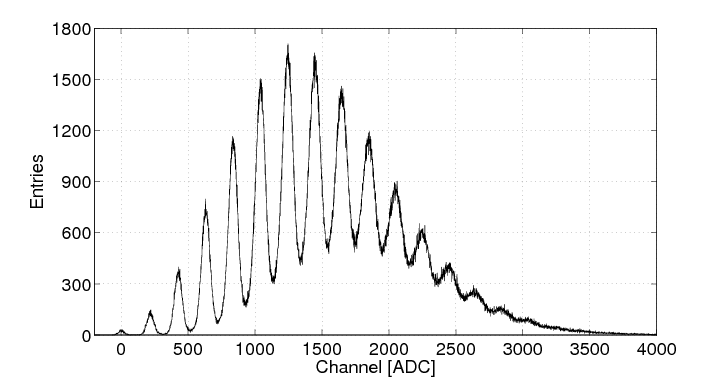
\includegraphics[width=\textwidth]{sipm_spectrum}};
    \node[label={[label distance=0.5cm,text depth=-1ex,rotate=90]above:pedestal}] at (-3, -1.5) {};
    \node[label={[label distance=0.5cm,text depth=-1ex,rotate=90]above:1 photo electron}] at (-2.6, -.5) {};
    \node[label={[label distance=0.5cm,text depth=-1ex,rotate=90]above:2 p.e.}] at (-2.2,-.8) {};
    \node[label={[label distance=0.5cm,text depth=-1ex,rotate=90]above:3 p.e.}] at (-1.8,0.2) {};
  \end{tikzpicture}
  \caption{%
    Sample spectrum of a \gls{sipm}.
    The first peak corresponds to the pedestal, followed by a series of peaks, each representing a number of simultaneously discharged cells.
    Since the uncertainties of the cells add up, the peaks get wider with increasing number of simultaneusly discharged cells.
  }
  \label{fig:cal_pedestal_spectrum}
\end{figure}

The spectrum of a \gls{sipm} consists of a series of peaks, the first peak corresponds to the pedestal, a gaussian distribution around the zero value.
The nature of this pedestal is the electronic noise and the current leaks generated by the electronic components.
The subsequent peaks correspond to simultaneously discharged \gls{sipm} cells and therefore to a number of photo electrons.
Since every peak corresponds to a number of simultaneously discharged cells, the distances between the position of the peaks corresponds to the gain of the \gls{sipm}.

\paragraph{Signal \& single photon resolution}
The signal in the readout is the sum of the signal when no avalanche occurrs -- also called pedestal -- and the avalanche signal
\begin{equation*}
	S_i = S_\text{pedestal} + i \cdot G,
\end{equation*}
where $G$ is the gain of signal in a \gls{sipm} and $i$ is the number of photo electrons or simultaneously discharged cells.

The fluctuations of the pedestal and gain uncertainties determine the single photon resolution:
\begin{equation*}
  \sigma(i)^2 = \sigma^2_\text{pedestal} + i \cdot \sigma^2_\text{gain},
\end{equation*}
where $i$ is the number of activated cells.
The fluctuations in the pedestal originate from unpredictable current leaks and readout electronics noise.
The uncertainties in the gains come from varying quenching resistances from cell to cell and the fluctuations during avalanche processes.

\paragraph{Dark rate, cross-talk \& after pulses} The dark rate is the event rate from avalanches generated by thermal or field mediated excitations of electrons in the silicon lattice and two correlated avalanche triggers: cross-talk and after pulses.

When the bias voltage is greater than the breakdown voltage, a charged carrier crossing the cell's p-n junction, can create a photon with sufficient energy to create an electron-hole pair.
The probability of this happening is of the order of $10^{-5}$, therefore for gains of the order of $10^5$, the number of these photons becomes significant\cite{1206.4154}.
It is important to point out, that these photons can propagate into nearby cells and initiate an avalanche.
This effect is called optical cross-talk.

During avalanches, electrons can be trapped in the Si-lattice and released later, producing a second avalanche after a characteristic time delay.
These avalanches are generally called after pulses.


\subsection{Determine the gain of a silicon photomultiplier}

Since the distance between neighboring peaks allows to compute the gain of the \glspl{sipm}, a method to identify the peaks, determine their positions and compute the distances is needed.
For this the part of the spectrum where the peaks are best visible is cut out.
\begin{figure}
  \centering
  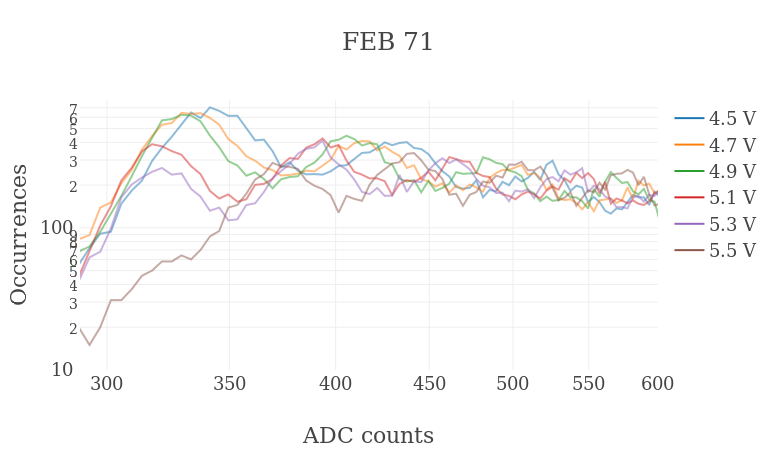
\includegraphics[width=\textwidth]{calibration/spectrum_cutout}
  \caption{%
    A small region of the spectrum has peaks, which are easy to identify.
  }
  \label{fig:spectrum_for_fit}
\end{figure}

First the positions of the peaks are estimated, using ROOT\cite{cern:root} and its TSpectrum class\cite{ROOT:TSpectrum}.
Three search parameters are used to find estimates: the width of the peaks, the bin size and the threshold.
Estimations are made by varying these parameters, each set of parameters leads to a search result with a number of peak candidates.

If the number of the estimated peak candidates is sufficently high, but doesn't exceed the number of expected peaks, a gaussian distribution is found to fit each peak candidate.
The resulting parameters are kept if the relative uncertainty of the position and the width is small\marginnote{$\sigma < 5\%$}.
Every set of search parameters leads therefore to a number of fitted peaks\marginnote{\ldots including fake peaks and missing some peaks sometimes!}.
The fitted positions are counted in a histogram, displayed in figure \ref{fig:cal_fitted_peaks}.

\begin{figure*}
  \centering
  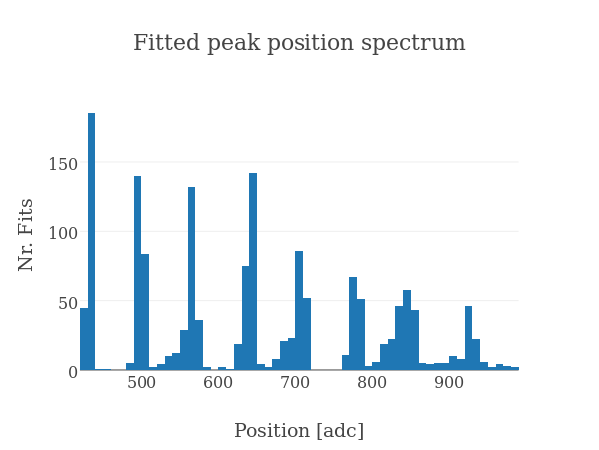
\includegraphics[width=.48\textwidth]{calibration/peak_spectrum}
  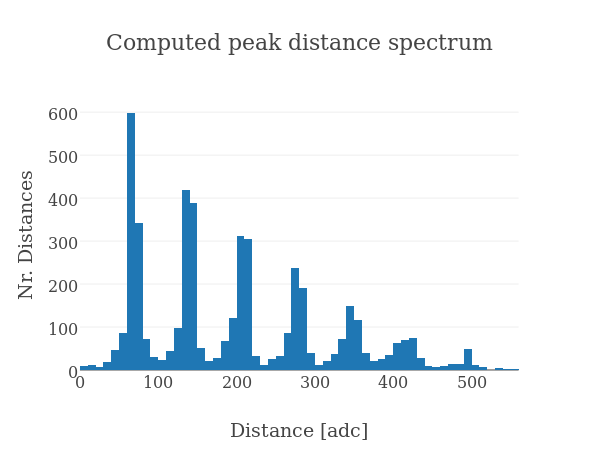
\includegraphics[width=.48\textwidth]{calibration/distances_spectrum}
  \caption{%
    The plot on the left shows the peak positions found for the given spectrum and different search parameters.
    The occurrences between the maxima show, that the search and fit method finds and registers fake peaks as well.
    The plot on the right displays the computed spectrum of distances.
    The first peak is the distance between two neigboring peaks.
    The second peak is the distance to the next proximate peaks, etc.
  }
  \label{fig:cal_fitted_peaks}
\end{figure*}

Since not only real peaks but fake peaks are identified and fitted as peaks, taking the mean and the standard deviation of the distances leads to undesired results.
This is avoided by computing the distances between the peaks for every set of fitted peaks.
Putting all these distances in a histogram -- as displayed in figure \ref{fig:cal_fitted_peaks} -- shows a series of clear features with decreasing height.
Assuming the number of found fake peaks is low, the most occurring distance is the distance between two neighboring peaks.
The position and width of a gaussian fitted around the greatest peak corresponds to the \gls{sipm}'s nominal gain and its uncertainty in \gls{adc} counts per photo electron -- see figure \ref{fig:cal_fitted_gain}.

\begin{figure}
  \centering
  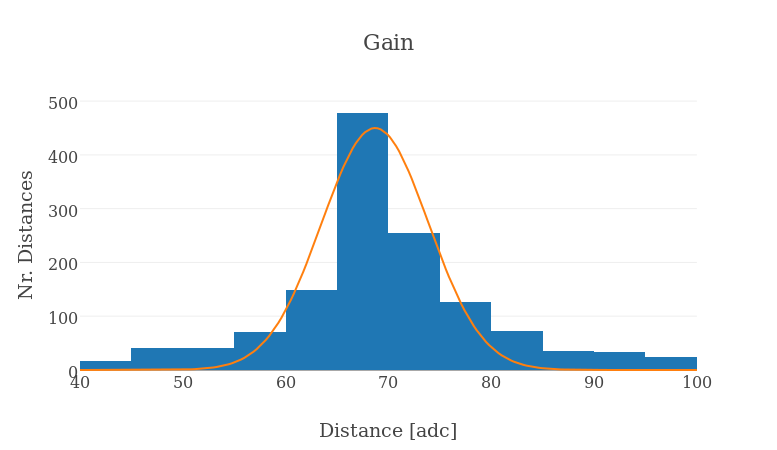
\includegraphics[width=\textwidth]{calibration/fitted_gain}
  \caption{%
    The plot displays the part of the histogram with the greatest peak and the fitted gaussian distribution around it.
  }
  \label{fig:cal_fitted_gain}
\end{figure}

\subsection{Dependency of the gain on the bias voltage}

When driven in Geiger mode, the cell of a \gls{sipm} behaves like a capacitance, accumulating charge -- which is responsible for the signal's gain -- due to a voltage supplied by the \gls{feb} charge
\begin{align}
  G &= \frac{C_\text{cell}}{e} (V_\text{bias} - V_\text{breakdown}) \label{eq:the_relation} \\
    &= \frac{C_\text{cell}}{e} V_\text{over voltage}  \\
    &\propto V_\text{over voltage},
\end{align}
where $C_\text{cell}$ is the capacitance of a cell, $e$ is the elementary electric charge,  $V_\text{breakdown}$ is the breakdown voltage of the \gls{sipm} and $V_\text{bias}$ is the bias voltage\marginnote{$V_\text{bias}$ is greater than $V_\text{breakdown}$ for \glspl{sipm} running in Geiger mode}.

This relation lets the observed spectrum and the gain depend heavily on the bias voltage.
A greater bias voltage leads to a greater charge stored in the \gls{sipm}'s cells and therefore to a greater discharge when the cell interacts with a photon.
This consequently leads to a higher gain.

The bias voltage of the \glspl{sipm} is generated by a manually trimmed stabilized power supply and a configurable \gls{dac} output voltage.
Since the trimmed output varies from \gls{feb} to \gls{feb} and the effective parameter used to calibrate the \glspl{crt} is the \gls{dac}'s setting, the gain is computed in dependence of the digital setting of the \gls{dac}.
The spectral change is displayed in figure \ref{fig:cal_changing_voltages}.

\begin{figure*}
  \centering
  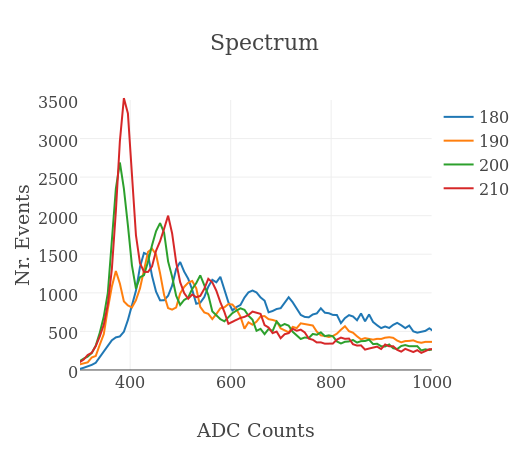
\includegraphics[width=.48\textwidth]{calibration/change_voltages}
  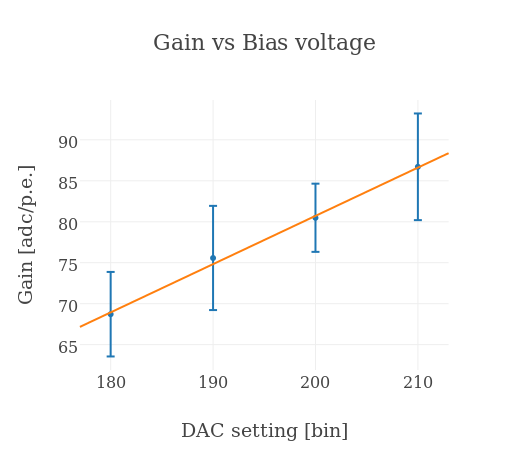
\includegraphics[width=.48\textwidth]{calibration/gain_vs_voltage}
  \caption{%
    The plot on the left displays spectra of a \gls{sipm} for increasing bias \gls{dac} output.
    It is clearly visible, that the spectrum shifts to the right with greater \gls{dac} setting.
    It is also visible, that the distance between the peaks increases with greater \gls{dac} setting.
    The plot on the right displays the dependence of the gain on the \gls{dac} setting.
  }
  \label{fig:cal_changing_voltages}
\end{figure*}

To determine this dependency, the bias voltage is changed by changing the setting responsible for the \gls{dac}'s output -- recall figure \ref{fig:voltage_generator}.
For every \gls{dac} setting, several sets of observations are made, the resulting relation is visible in figure \ref{fig:cal_changing_voltages}.
Even if the uncertainty of the gain is high at every observation point, a linear dependency can be guessed.

\subsection{The spectra of an uncalibrated panel vs. a calibrated panel}

The observed spectra vary from \gls{sipm} to \gls{sipm}.
For ideal components, fixing the bias voltage to a certain value for all \glspl{sipm} solves the problem.
In the case of real components a change in the spectrum is clearly visible, as displayed in figure \ref{fig:cal_uncalibrated_spectra}.

\begin{figure}
  \centering
  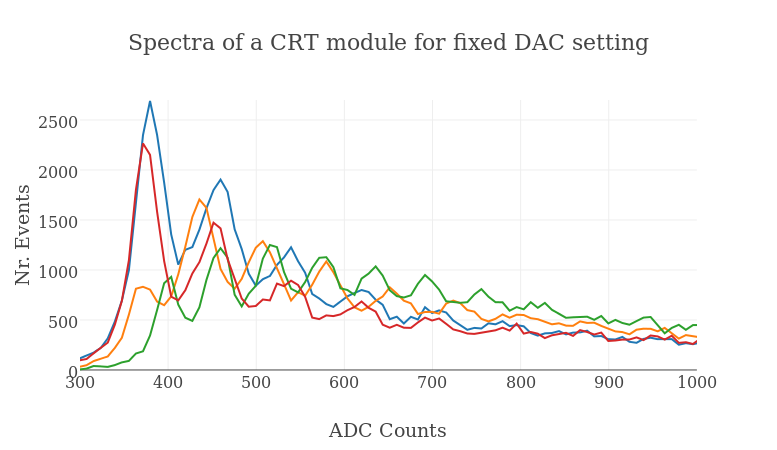
\includegraphics[width=\textwidth]{calibration/uncalibrated_spectra}
  \caption{%
    The spectra of 4 channels of the same \gls{crt} module are displayed.
    Every color represents one of the observed channels.
  }
  \label{fig:cal_uncalibrated_spectra}
\end{figure}

The gains of the \glspl{sipm} are computed and displayed in the left plot of figure \ref{fig:cal_vs_uncal} to visualize the distribution of gains in within a \gls{crt} module for fixed bias voltages.

With the aim to improve the spread of gains within a \gls{crt} module and improve therefore the uncertainty of the gain, the dependency of the gain on the bias voltage is computed for every \gls{sipm} of the \gls{crt} module.
The obtained curves are plotted in figure \ref{fig:cal_dependencies}.

\begin{figure}
  \centering
  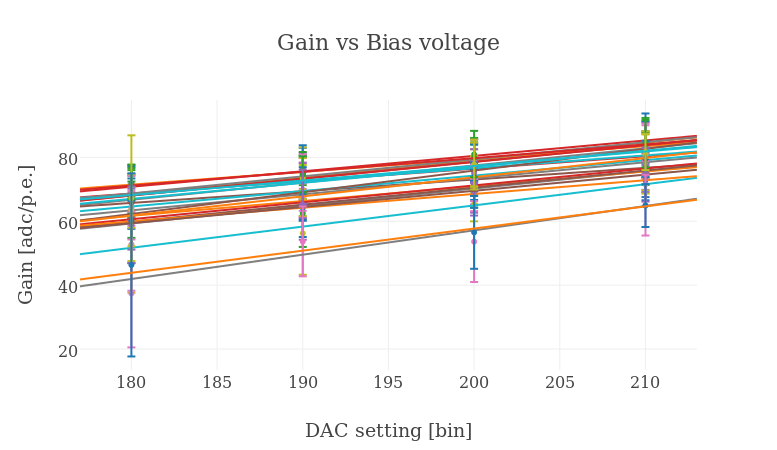
\includegraphics[width=\textwidth]{calibration/dependencies_run_1}
  \caption{%
    Change in gain in dependency of the \gls{dac} setting.
    Every colored line represents a different channel.
  }
  \label{fig:cal_dependencies}
\end{figure}

The inclination of the resulting slopes are similar for all the \glspl{sipm}.
The interval of configurable gains is narrow in within the given range of bias settings.
Due to the spread of the slope's position the interval of achievable gains for an uniform distribution is further reduced.

Using the computed dependencies and a simplified version of relation \ref{eq:the_relation}\marginnote{%
  $G = a \cdot \text{bias} + b \to \text{bias} = \frac{G-b}{a} $
} the settings for the biasing \gls{dac} is computed for every \gls{sipm}, with the aim to reduce the dispersion of gains within a module.

To test the sensitivity of the calibration, the bias settings are computed for three different gain within the attainable range: 75, 85 and 65 \gls{adc} counts per photo electron.
A set of observations is made for every set of computed settings and the gains are computed and counted for every \gls{sipm}.
The distributions are displayed in the right plot of figure \ref{fig:cal_vs_uncal}.

\begin{figure*}
  \centering
  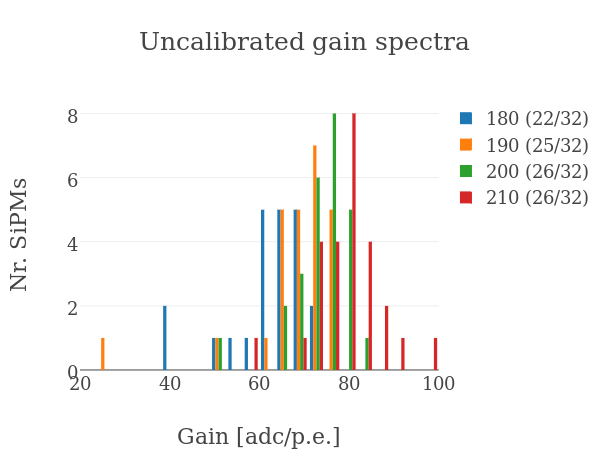
\includegraphics[width=.48\textwidth]{calibration/vorher}
  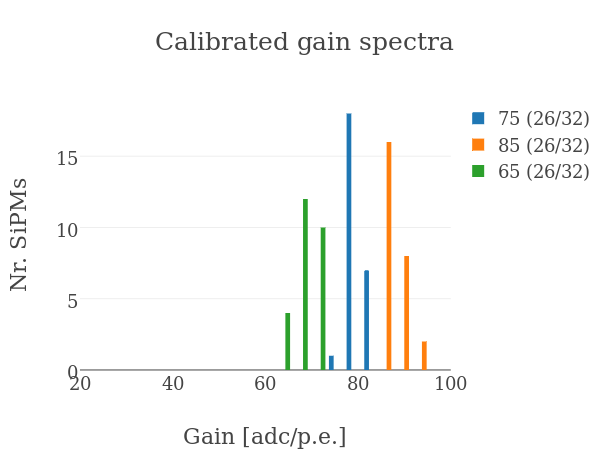
\includegraphics[width=.48\textwidth]{calibration/nacher}
  \caption{%
    The plot on the left shows the spectrum of computed gains for fixed \gls{dac} settings for every \gls{sipm}.
    The plot on the right displays the distribution of gains after the calibration process.
    To make the change more visible, the same range for the x axis is used.
  }
  \label{fig:cal_vs_uncal}
\end{figure*}

An important reduction of the spread of gains is observable in the plots of figure \ref{fig:cal_vs_uncal}.

For comparison with the uncalibrated spectra, the observed spectra for fixed nominal gains are displayed in figure \ref{fig:cal_vs_uncal_spectrum}.

\begin{figure*}
  \centering
  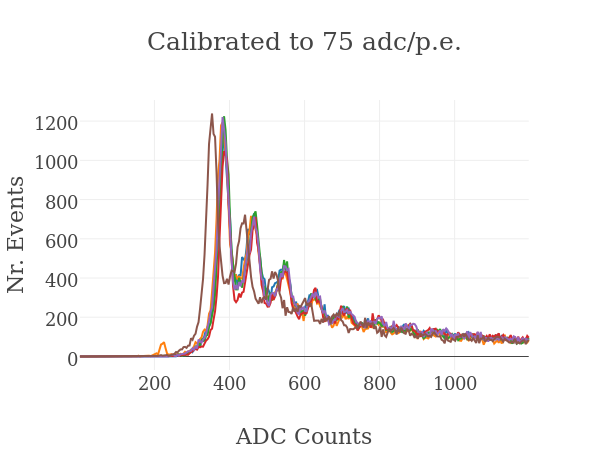
\includegraphics[width=.32\textwidth]{calibration/spectrum_75}
  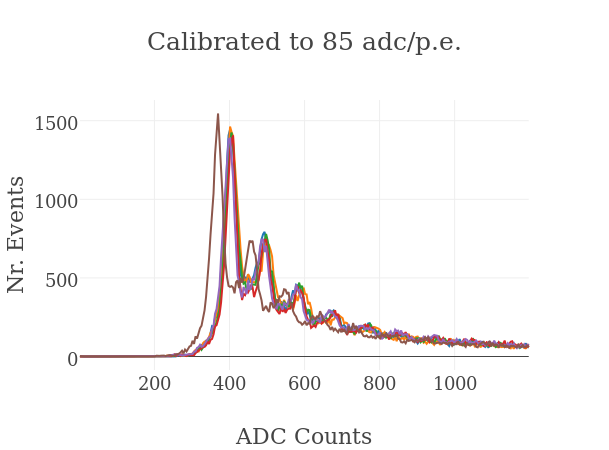
\includegraphics[width=.32\textwidth]{calibration/spectrum_85}
  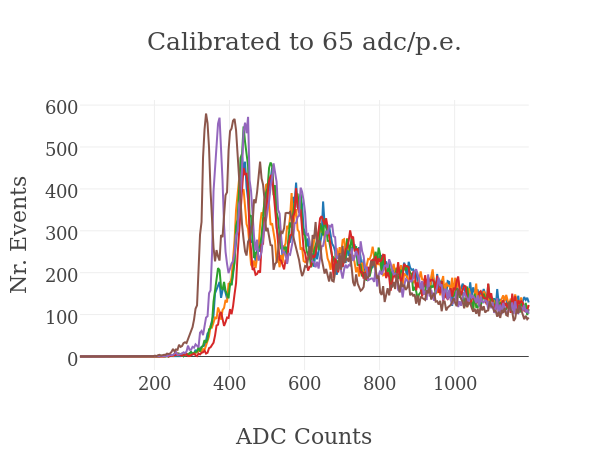
\includegraphics[width=.32\textwidth]{calibration/spectrum_65}
  \caption{%
    Observed spectra after calibration process.
  }
  \label{fig:cal_vs_uncal_spectrum}
\end{figure*}

An improvement in the spectra's uniformity in comparison to the uncalibrated spectra shown in figure \ref{fig:cal_uncalibrated_spectra} is visible.
